% Options for packages loaded elsewhere
\PassOptionsToPackage{unicode}{hyperref}
\PassOptionsToPackage{hyphens}{url}
%
\documentclass[
  man,floatsintext]{apa6}
\usepackage{amsmath,amssymb}
\usepackage{iftex}
\ifPDFTeX
  \usepackage[T1]{fontenc}
  \usepackage[utf8]{inputenc}
  \usepackage{textcomp} % provide euro and other symbols
\else % if luatex or xetex
  \usepackage{unicode-math} % this also loads fontspec
  \defaultfontfeatures{Scale=MatchLowercase}
  \defaultfontfeatures[\rmfamily]{Ligatures=TeX,Scale=1}
\fi
\usepackage{lmodern}
\ifPDFTeX\else
  % xetex/luatex font selection
\fi
% Use upquote if available, for straight quotes in verbatim environments
\IfFileExists{upquote.sty}{\usepackage{upquote}}{}
\IfFileExists{microtype.sty}{% use microtype if available
  \usepackage[]{microtype}
  \UseMicrotypeSet[protrusion]{basicmath} % disable protrusion for tt fonts
}{}
\makeatletter
\@ifundefined{KOMAClassName}{% if non-KOMA class
  \IfFileExists{parskip.sty}{%
    \usepackage{parskip}
  }{% else
    \setlength{\parindent}{0pt}
    \setlength{\parskip}{6pt plus 2pt minus 1pt}}
}{% if KOMA class
  \KOMAoptions{parskip=half}}
\makeatother
\usepackage{xcolor}
\usepackage{graphicx}
\makeatletter
\def\maxwidth{\ifdim\Gin@nat@width>\linewidth\linewidth\else\Gin@nat@width\fi}
\def\maxheight{\ifdim\Gin@nat@height>\textheight\textheight\else\Gin@nat@height\fi}
\makeatother
% Scale images if necessary, so that they will not overflow the page
% margins by default, and it is still possible to overwrite the defaults
% using explicit options in \includegraphics[width, height, ...]{}
\setkeys{Gin}{width=\maxwidth,height=\maxheight,keepaspectratio}
% Set default figure placement to htbp
\makeatletter
\def\fps@figure{htbp}
\makeatother
\setlength{\emergencystretch}{3em} % prevent overfull lines
\providecommand{\tightlist}{%
  \setlength{\itemsep}{0pt}\setlength{\parskip}{0pt}}
\setcounter{secnumdepth}{-\maxdimen} % remove section numbering
% Make \paragraph and \subparagraph free-standing
\ifx\paragraph\undefined\else
  \let\oldparagraph\paragraph
  \renewcommand{\paragraph}[1]{\oldparagraph{#1}\mbox{}}
\fi
\ifx\subparagraph\undefined\else
  \let\oldsubparagraph\subparagraph
  \renewcommand{\subparagraph}[1]{\oldsubparagraph{#1}\mbox{}}
\fi
\newlength{\cslhangindent}
\setlength{\cslhangindent}{1.5em}
\newlength{\csllabelwidth}
\setlength{\csllabelwidth}{3em}
\newlength{\cslentryspacingunit} % times entry-spacing
\setlength{\cslentryspacingunit}{\parskip}
\newenvironment{CSLReferences}[2] % #1 hanging-ident, #2 entry spacing
 {% don't indent paragraphs
  \setlength{\parindent}{0pt}
  % turn on hanging indent if param 1 is 1
  \ifodd #1
  \let\oldpar\par
  \def\par{\hangindent=\cslhangindent\oldpar}
  \fi
  % set entry spacing
  \setlength{\parskip}{#2\cslentryspacingunit}
 }%
 {}
\usepackage{calc}
\newcommand{\CSLBlock}[1]{#1\hfill\break}
\newcommand{\CSLLeftMargin}[1]{\parbox[t]{\csllabelwidth}{#1}}
\newcommand{\CSLRightInline}[1]{\parbox[t]{\linewidth - \csllabelwidth}{#1}\break}
\newcommand{\CSLIndent}[1]{\hspace{\cslhangindent}#1}
\ifLuaTeX
\usepackage[bidi=basic]{babel}
\else
\usepackage[bidi=default]{babel}
\fi
\babelprovide[main,import]{english}
% get rid of language-specific shorthands (see #6817):
\let\LanguageShortHands\languageshorthands
\def\languageshorthands#1{}
% Manuscript styling
\usepackage{upgreek}
\captionsetup{font=singlespacing,justification=justified}

% Table formatting
\usepackage{longtable}
\usepackage{lscape}
% \usepackage[counterclockwise]{rotating}   % Landscape page setup for large tables
\usepackage{multirow}		% Table styling
\usepackage{tabularx}		% Control Column width
\usepackage[flushleft]{threeparttable}	% Allows for three part tables with a specified notes section
\usepackage{threeparttablex}            % Lets threeparttable work with longtable

% Create new environments so endfloat can handle them
% \newenvironment{ltable}
%   {\begin{landscape}\centering\begin{threeparttable}}
%   {\end{threeparttable}\end{landscape}}
\newenvironment{lltable}{\begin{landscape}\centering\begin{ThreePartTable}}{\end{ThreePartTable}\end{landscape}}

% Enables adjusting longtable caption width to table width
% Solution found at http://golatex.de/longtable-mit-caption-so-breit-wie-die-tabelle-t15767.html
\makeatletter
\newcommand\LastLTentrywidth{1em}
\newlength\longtablewidth
\setlength{\longtablewidth}{1in}
\newcommand{\getlongtablewidth}{\begingroup \ifcsname LT@\roman{LT@tables}\endcsname \global\longtablewidth=0pt \renewcommand{\LT@entry}[2]{\global\advance\longtablewidth by ##2\relax\gdef\LastLTentrywidth{##2}}\@nameuse{LT@\roman{LT@tables}} \fi \endgroup}

% \setlength{\parindent}{0.5in}
% \setlength{\parskip}{0pt plus 0pt minus 0pt}

% Overwrite redefinition of paragraph and subparagraph by the default LaTeX template
% See https://github.com/crsh/papaja/issues/292
\makeatletter
\renewcommand{\paragraph}{\@startsection{paragraph}{4}{\parindent}%
  {0\baselineskip \@plus 0.2ex \@minus 0.2ex}%
  {-1em}%
  {\normalfont\normalsize\bfseries\itshape\typesectitle}}

\renewcommand{\subparagraph}[1]{\@startsection{subparagraph}{5}{1em}%
  {0\baselineskip \@plus 0.2ex \@minus 0.2ex}%
  {-\z@\relax}%
  {\normalfont\normalsize\itshape\hspace{\parindent}{#1}\textit{\addperi}}{\relax}}
\makeatother

% \usepackage{etoolbox}
\makeatletter
\patchcmd{\HyOrg@maketitle}
  {\section{\normalfont\normalsize\abstractname}}
  {\section*{\normalfont\normalsize\abstractname}}
  {}{\typeout{Failed to patch abstract.}}
\patchcmd{\HyOrg@maketitle}
  {\section{\protect\normalfont{\@title}}}
  {\section*{\protect\normalfont{\@title}}}
  {}{\typeout{Failed to patch title.}}
\makeatother

\usepackage{xpatch}
\makeatletter
\xapptocmd\appendix
  {\xapptocmd\section
    {\addcontentsline{toc}{section}{\appendixname\ifoneappendix\else~\theappendix\fi\\: #1}}
    {}{\InnerPatchFailed}%
  }
{}{\PatchFailed}
\keywords{social cognition, individual differences, gaze cues, cognitive modeling\newline\indent Word count: xxx}
\usepackage{lineno}

\linenumbers
\usepackage{csquotes}
\usepackage{setspace}
\captionsetup[figure]{font={stretch=1}}
\ifLuaTeX
  \usepackage{selnolig}  % disable illegal ligatures
\fi
\IfFileExists{bookmark.sty}{\usepackage{bookmark}}{\usepackage{hyperref}}
\IfFileExists{xurl.sty}{\usepackage{xurl}}{} % add URL line breaks if available
\urlstyle{same}
\hypersetup{
  pdftitle={Variation in gaze understanding across the life span: A process-level perspective},
  pdfauthor={Julia Prein1, Manuel Bohn1,2, Luke Maurits1, Annika Werwach1, \& Daniel B. M. Haun1},
  pdflang={en-EN},
  pdfkeywords={social cognition, individual differences, gaze cues, cognitive modeling},
  hidelinks,
  pdfcreator={LaTeX via pandoc}}

\title{Variation in gaze understanding across the life span: A process-level perspective}
\author{Julia Prein\textsuperscript{1}, Manuel Bohn\textsuperscript{1,2}, Luke Maurits\textsuperscript{1}, Annika Werwach\textsuperscript{1}, \& Daniel B. M. Haun\textsuperscript{1}}
\date{}


\shorttitle{modeling variation in gaze understanding}

\authornote{

The authors made the following contributions. Julia Prein: Conceptualization, Methodology, Software, Investigation, Formal Analysis, Writing - Original Draft Preparation, Writing - Review \& Editing; Manuel Bohn: Conceptualization, Formal Analysis, Writing - Original Draft Preparation, Writing - Review \& Editing; Luke Maurits: Formal Analysis, Writing - Review \& Editing; Annika Werwach: Methodology, Investigation, Writing - Review \& Editing; Daniel B. M. Haun: Supervision, Writing - Review \& Editing.

Correspondence concerning this article should be addressed to Julia Prein, Max Planck Institute for Evolutionary Anthropology, Deutscher Platz 6, 04103 Leipzig, Germany. E-mail: \href{mailto:julia_prein@eva.mpg.de}{\nolinkurl{julia\_prein@eva.mpg.de}}

}

\affiliation{\vspace{0.5cm}\textsuperscript{1} Department of Comparative Cultural Psychology, Max Planck Institute for Evolutionary Anthropology, Leipzig, Germany\\\textsuperscript{2} Institute of Psychology, Leuphana University Lüneburg, Germany}

\abstract{%
Abstract
}



\begin{document}
\maketitle

\hypertarget{introduction}{%
\section{Introduction}\label{introduction}}

\begin{itemize}
\tightlist
\item
  why do we care about developmental trajectory? ref to stat learning paper
\item
  variation
\end{itemize}

\hypertarget{why-do-we-need-gaze-understanding}{%
\subsection{Why do we need gaze understanding?}\label{why-do-we-need-gaze-understanding}}

How do humans learn about their environment and navigate through their social surroundings?
One possibility to extract information from the environment is through following others' focus of attention.
Building a common ground is considered especially important in communicative interactions and shared activities (Tomasello, Hare, Lehmann, \& Call, 2007).

\hypertarget{how-does-gaze-following-emerge}{%
\subsection{How does gaze following emerge?}\label{how-does-gaze-following-emerge}}

Existing studies operationalize gaze following as the ability to follow another agent's line of sight.
As one of the most fundamental social-cognitive abilities, it has been extensively studied in infancy and early childhood.
Infants as young as six months can attune their gaze to that of another agent (D'Entremont, Hains, \& Muir, 1997).
At the end of their first year of life, infants can follow gaze to locations outside their current visual field and move themselves to gain proper perceptual access (Moll \& Tomasello, 2004).

While the emergence of gaze following has been well established, less is known about the developmental trajectory throughout childhood and adolescence.
One possibility is that our social-cognitive ability in question is fully developed once emerged in infancy.However, many cognitive abilities develop with age (e.g., working memory, Gathercole, Pickering, Ambridge, \& Wearing, 2004).
Similarly, visual processing appears to improve with age.
Therefore, children could potentially improve in gaze following, fine-tuning the performance of the already existing skill.

\hypertarget{the-scope-of-infants-gaze-following-ability}{%
\subsection{The scope of infants' gaze following ability}\label{the-scope-of-infants-gaze-following-ability}}

Though these studies suggest that young infants can align their visual attention to another's line of sight, it does not necessarily include understanding the intentions of the other agent.
Infants could simply attune their orientation or be attracted by others' gaze without processing what exactly the other is seeing (cf.~Butterworth \& Jarrett's ecological and geometric mechanism, Butterworth and Jarrett (1991){]}. Therefore, it is crucial to study children's intentional understanding of gaze.

Moore, Angelopoulos, and Bennett (1997) showed that 9-month-olds followed an agent's gaze more, when it was accompanied by a dynamic head turn in comparison to a static head turn.

In a hiding game with two search locations, Povinelli, Reaux, Bierschwale, Allain, and Simon (1997) found that three-year-olds used gaze as a cue to locate the reward, while two-year-olds performed at chance level.

In a similar object choice paradigm with two containers, Behne, Carpenter, and Tomasello (2005) investigated whether infants understand the communicative intent behind pointing and gaze cues.
In contrast to Povinelli et al. (1997), they found that already 14-month-olds used the agent's cues to select an object.
In conditions with absent-minded `cues', infants performed around chance.
This could be interpreted as infants recognizing the nature of this joint activity: namely, that the adult's behavior was beneficial and relevant for their object choice.

\hypertarget{head-vs-eye-direction}{%
\subsubsection{Head vs eye direction}\label{head-vs-eye-direction}}

It is important to note that in many existing gaze conditions, the experimenter shifted their eyes and head in synchrony (e.g., Behne et al. (2005)).
Instead of pointing towards gaze understanding, a critic could claim that the results can be explained by face direction alone.

A handful of studies approached this potential confound by separately manipulating head and eye movement.
Brooks and Meltzoff (2002) implemented a comparison between eye and head orientation and found that 14-month-olds were sensitive to open versus closed eyes.

Investigating the `cooperative eye hypothesis', Tomasello et al. (2007) implemented six conditions, in which an experimenter oriented towards the ceiling with their eyes only, head only (eyes closed), both head and eyes, or neither.
They found that human infants relied more on the eye movement, while chimpanzees paid more attention to the head movement.

Importantly, the subjects were not presented with an object choice but their attention orientation was measured.

\begin{itemize}
\item
  (Raviv \& Arnon, 2018)
\item
  (Astor \& Gredebäck, 2022)
\item
  (Colombo, 2001)
\item
  (Scaife \& Bruner, 1975)
\item
  (Itakura \& Tanaka, 1998)
\item
  (Carpenter, Nagell, \& Tomasello, 1998) ``Several other studies have attempted to determine more precisely the cue that infants are using when they follow the gaze direction of others, that is, whether they use adults' head or eye orientation. In tasks comparing infants' responses when the experimenters turned their head and eyes together to targets with their responses when the experimenters directed their eyes to the targets but their head remained facing forward, Corkum and Moore (1995), Lempers (1979), and Lempers, Flavell, and Flavell (1977) all found that only infants age 12 months and older responded correctly when eyes and head were oriented in the same direction and that infants at all ages (i.e., through 19 months) performed poorly when eye and head direction diverged'' (p.10-11) object choice.
\item
  (Silverstein, Feng, Westermann, Parise, \& Twomey, 2021) for vertical plane
\item
  (Zhang, Zhang, Zhang, Tang, \& Liu, 2019)
\item
  (Frischen, Bayliss, \& Tipper, 2007)
\item
  (Lee, Eskritt, Symons, \& Muir, 1998)
\item
  (Coelho, George, Conty, Hugueville, \& Tijus, 2006)
\end{itemize}

\hypertarget{aim-of-the-current-project}{%
\subsection{Aim of the current project}\label{aim-of-the-current-project}}

\hypertarget{developmental-trajectory-measuring-modeling-individual-differences}{%
\subsubsection{Developmental trajectory, measuring \& modeling individual differences}\label{developmental-trajectory-measuring-modeling-individual-differences}}

In this study, we were interested in the developmental trajectory of gaze understanding.
While we expect the younger children to be able to follow gaze, we aimed at assessing the differentiation of their social-cognitive ability.
Our goal was \emph{not} to establish the youngest age at which children understand gaze cues.
Rather, we wanted to examine how that ability changes with age.

In our study, we focused on the communicative intents of gaze: we asked children to locate a target by following an agent's gaze.
While language demands were kept low, the participants had to actively respond and, therefore, make use of the presented gaze cue.

A unique contribution of this study is the richness of the data set.
Methodological challenges arise when trying to compare data across ages from qualitatively and quantitatively different study tasks.
We could circumvent these issues by applying the exact same task for the entire life span.

\hypertarget{lifespan}{%
\section{Lifespan}\label{lifespan}}

\begin{itemize}
\tightlist
\item
  development \& individual differences in gaze understanding
\item
  verweis methods paper reliable differences kinder \& adults.
\item
  kontinuerliche, systematische variation, wodrin? =\textgreater{} model
\end{itemize}

\url{https://osf.io/6yjz3}

\begin{table}[tbp]

\begin{center}
\begin{threeparttable}

\caption{\label{tab:lifespan_sample}}

\begin{tabular}{lllll}
\toprule
Age group & \multicolumn{1}{c}{n} & \multicolumn{1}{c}{Age mean} & \multicolumn{1}{c}{Age range} & \multicolumn{1}{c}{Age SD}\\
\midrule
3.00 & 19 (7 female) & 3.62 & 3.04 - 3.99 & 0.31\\
4.00 & 17 (9 female) & 4.45 & 4.05 - 4.91 & 0.30\\
5.00 & 22 (13 female) & 5.56 & 5.08 - 5.99 & 0.31\\
6.00 & 24 (16 female) & 6.50 & 6.1 - 6.99 & 0.28\\
7.00 & 39 (20 female) & 7.48 & 7.04 - 7.95 & 0.25\\
8.00 & 41 (20 female) & 8.46 & 8.03 - 8.98 & 0.27\\
9.00 & 56 (29 female) & 9.46 & 9.01 - 9.96 & 0.28\\
10.00 & 35 (22 female) & 10.49 & 10.01 - 11 & 0.28\\
11.00 & 54 (26 female) & 11.43 & 11.01 - 11.96 & 0.28\\
12.00 & 43 (19 female) & 12.41 & 12.01 - 12.99 & 0.30\\
13.00 & 42 (19 female) & 13.50 & 13.09 - 13.99 & 0.27\\
14.00 & 20 (14 female) & 14.37 & 14.05 - 14.98 & 0.23\\
15.00 & 21 (11 female) & 15.56 & 15.05 - 15.98 & 0.30\\
16.00 & 19 (10 female) & 16.51 & 16.17 - 16.97 & 0.24\\
17.00 & 19 (10 female) & 17.53 & 17.01 - 17.95 & 0.28\\
18.00 & 2 (0 female) & 18.00 & 18 - 18 & 0.00\\
19.00 & 5 (4 female) & 19.00 & 19 - 19 & 0.00\\
20.00 & 40 (25 female) & 23.02 & 20 - 29 & 2.77\\
30.00 & 40 (21 female) & 34.42 & 30 - 39 & 3.00\\
40.00 & 40 (24 female) & 44.17 & 40 - 49 & 2.92\\
50.00 & 40 (21 female) & 54.38 & 50 - 59 & 3.04\\
60.00 & 40 (21 female) & 63.73 & 60 - 69 & 2.56\\
70.00 & 40 (20 female) & 72.75 & 70 - 79 & 2.44\\
\bottomrule
\end{tabular}

\end{threeparttable}
\end{center}

\end{table}

\hypertarget{participants}{%
\subsection{Participants}\label{participants}}

We collected data from a remote child, teenager and adult sample.
For the remote child and teenager sample, we recruited participants via an internal database consisting of families living in Leipzig, Germany, who volunteered to participate in child development studies and indicated an interest in online studies.

The remote child and teenager sample consisted of 471 participants.
Children and teenagers in our sample grow up in an industrialized, urban Central-European context.
Information on socioeconomic status was not formally recorded, although the majority of families come from mixed, mainly mid to high socioeconomic backgrounds with high levels of parental education.

Adults were recruited via \emph{Prolific} (Palan \& Schitter, 2018).
\emph{Prolific} is an online participant recruitment service from the University of Oxford with a predominantly European and US-American subject pool.
Participants consisted of 240 English-speaking adults that reported to have normal or corrected-to-normal vision.
For further information on age and gender of participants, see Table 1.

For completing the study, subjects were paid above the fixed minimum wage (on average £10.00 per hour; see Supplements for further detail).

\hypertarget{materials}{%
\subsection{Materials}\label{materials}}

We used the continuous version of the TANGO (Prein, Bohn, Kalinke, \& Haun, 2022).
The task was presented as an interactive web application (see Figure \ref{fig:fig1}; live demo \href{https://ccp-odc.eva.mpg.de/tango-demo/.}{https://ccp-odc.eva.mpg.de/tango-demo/}; source code \url{https://github.com/ccp-eva/tango-demo}).
The TANGO showed satisfactory internal consistency and retest reliability {[}with reliability estimates \emph{Pearson's r} ranging from .7 to .8 for the continuous task version; Prein et al. (2022){]}.

Each trial presented an agent standing in a window, watching a balloon (\emph{i.e.}, target) falling to the ground.
The target then fell behind a hedge (continuous task version).
The agent's gaze followed the target's trajectory: pupil and iris moved so that their center aligned with the target center.
In test trials, the target flight was covered so that participants could not see where the target landed.
Participants' task was to locate the target by tracking the agent's gaze.
They could respond by touching on the screen.

Four familiarization trials ensured that participants understood the task and felt comfortable with the response format.
Then, 15 test trials followed.
Completing the 19 trials took approximately 5-10 minutes.

The outcome measure was imprecision, defined as the absolute difference between the target center and the x coordinate of the participant's click.
Target coordinates were randomly generated during runtime.
Each target bin, as well as all agents and target colors, occurred equally often and and did not appear in more than two consecutive trials.



\begin{figure}

{\centering 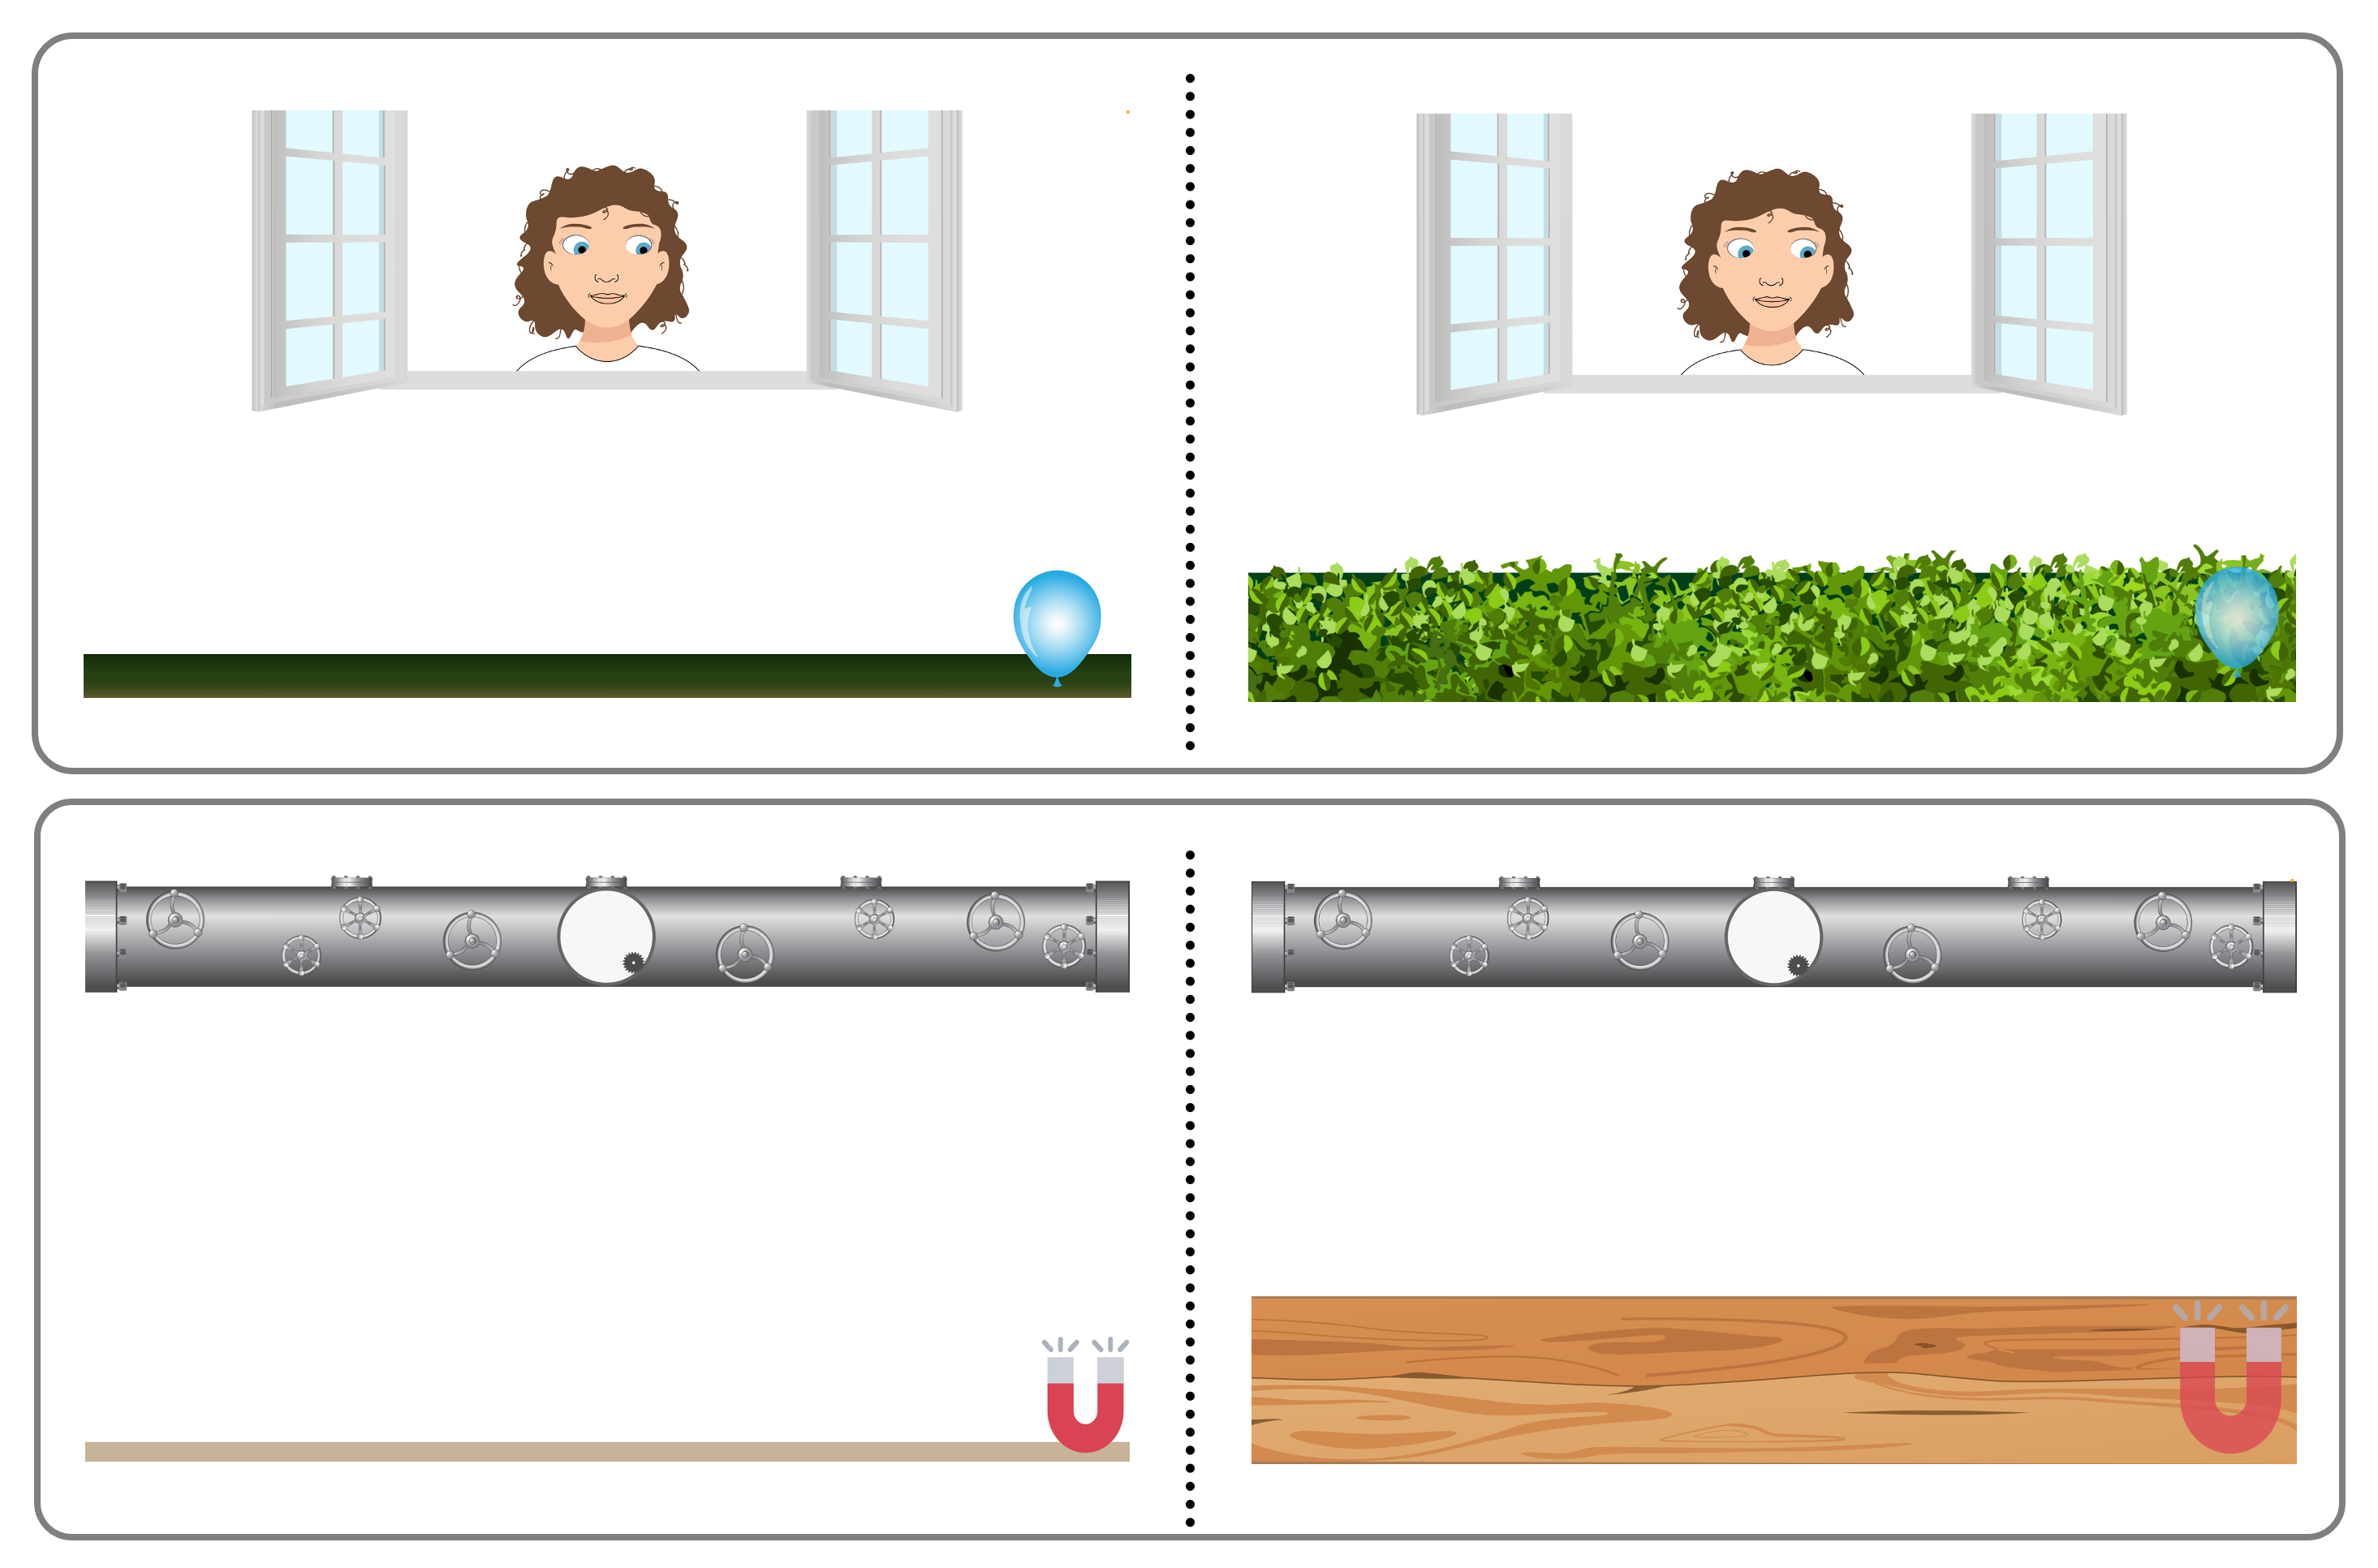
\includegraphics[width=1\linewidth]{../figures/procedure} 

}

\caption{\textbf{Setup of the TANGO and Magnet tasks}. (A) TANGO: Gaze understanding task. The agent stands in a window with the target in front of them. A hedge grows and covers the target. The target falls to a random location on the ground. The agent's eyes track the movement of the target. (B) Magnet task: non-social vector estimation.}\label{fig:fig1}
\end{figure}

\hypertarget{procedure}{%
\subsection{Procedure}\label{procedure}}

Children and teenagers received a personalized link to the study website.
Caregivers were asked to provide technical support whenever needed, while explicitly being reminded to not help their children in responding.
Webcam videos were recorded whenever consented and technically feasible, in order to monitor whether children and teenagers responded on their own.

\hypertarget{analysis}{%
\subsection{Analysis}\label{analysis}}

All test trials without voice-over description were included in our analyses.
We ran all analyses in R version 4.3.0 (2023-04-21) (R Core Team, 2022).
Regression models were fit as Bayesian generalized linear mixed models (GLMMs) with default priors for all analyses, using the function \texttt{brm} from the package \texttt{brms} (Bürkner, 2017, 2018).

To estimate the developmental trajectory of gaze understanding and the effect of data collection mode, we fit a GLMM predicting the task performance in each trial by age (in months, z-transformed), in \texttt{R:\ imprecision\ \textasciitilde{}\ age\_centered}).

Imprecision was defined as the absolute click distance between the target center and the click X coordinate, scaled according to target widths, and modeled by a \texttt{lognormal} distribution.
We inspected the posterior distribution (mean and 95\% Confidence Interval (CI)) for the age and data collection estimates.

\hypertarget{results}{%
\subsection{Results}\label{results}}



\begin{figure}

{\centering 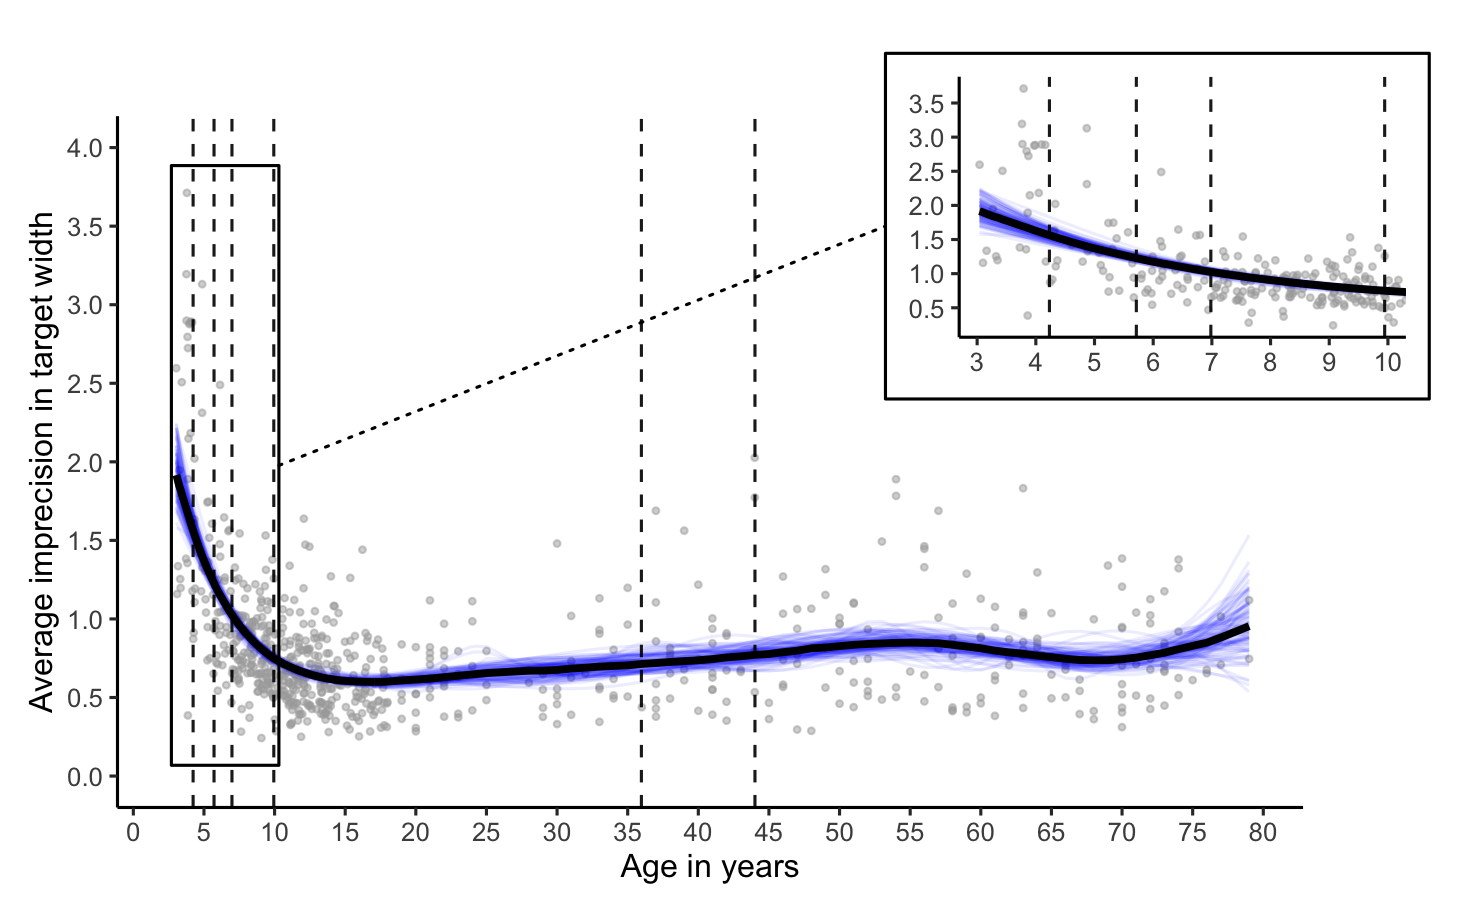
\includegraphics[width=1\linewidth]{../figures/lifespan_plot} 

}

\caption{\textbf{Differentiation in gaze understanding}. Performance is measured as imprecision, i.e., the absolute distance between the target's center and the participant's click (averaged across trials). The unit of imprecision is counted in the width of the target, i.e., a participant with imprecision of 1 clicked on average one target width to the left or right of the true target center.}\label{fig:fig2}
\end{figure}

\hypertarget{discussion}{%
\subsection{Discussion}\label{discussion}}

Three-year-olds were surprisingly inaccurate in their responses.
One possible explanation could be that they simply lacked the ability to complete the task, potentially due to issues in gaze following.
Contrasting our results with previous findings on infant gaze following, this explanation is unlikely.
A more likely explanation would be that children were able to follow the agent's gaze but struggled to translate this implicit understanding into active behavior.

Another point to keep in mind is that we used subtle eye movements as cues.
Many existing studies let the agents move eye and head in parallel, therefore establishing a confound with greater (head) movement.
Relying exclusively on the eye movement might be trickier for children than when presented with a combined eye and head orientation.

The performance of the youngest children seems more consistent with performance demands than with a failure in gaze following.

\hypertarget{computational-cognitive-model}{%
\section{Computational cognitive model}\label{computational-cognitive-model}}

In a previous study, we have shown that the inter-individual variation in gaze understanding is reliable (Prein et al. (2022)).
Now, we asked ourselves what varies between participants on a process-level and how this changes with age.
To answer this question, we aimed to formalize the process of gaze understanding in a computational cognitive model.
The model seeks to explain how participants solve the TANGO task.

Computational modeling frameworks allow researcher to establish mechanistic explanations of psychological phenomena and form testable predictions (Grahek, Schaller, \& Tackett, 2021).
As formal, mathematical accounts of the psychological process in question, they force researchers to accurately and comprehensively state all underlying assumptions (Simmering, Triesch, Deák, \& Spencer, 2010).
In addition, models can be used to simulate and predict behavior as it would be expected in novel experimental manipulations.
This can then in turn be compared to empirically observed behavior and can, for example, demonstrate assumptions of the model to be false.

The model assumes that participants estimate the agent's eye center and observe the current location of the pupil center.
These two point estimates are then used to calculate a vector that points towards the attentional focus of the agent.
Our model assumes that participants sample from a distribution around the true gaze vector.
Individual differences could now be explained as more narrow or wider distribution around the true gaze vector (i.e., amount of deviation).
This could represent participants' level of uncertainty in estimating the agent's attentional focus: the wider the distribution around the true gaze vector, the less precise participants estimate the focus of attention.
This is the key parameter in our model: this so-called inferential component describes how accurately the participant infers the attentional focus based upon the state of the agent's pupil.

However, participants who are very imprecise in locating the attentional focus of the agent could be less likely to make use of the eye information in the first place.
To accomodate this, we created an alternative model that estimates the probability that a participant engages in random guessing.

With this approach, we can formalize whether (A) a participant makes use of the available gaze information at all, and (B) how accurate they are, if they do pay attention to the agent's eyes.
We expect a dual developmental process.
The older children get, the more likely they are to use the gaze cues and the more precise they get in doing so.

The geometry of the estimated gaze vector and the sampling of a distribution around this vector lead to interesting, testable group-level predictions.
As the pupil location varies, a fixed amount of uncertainty about the eye angle corresponds to a varying amount of uncertainty in the estimated focus of attention (i.e., the target location).
This could be thought of as a ``headlight distribution'': when the agent's eye gaze is directed centrally to the ground in front of them, the distribution from which participants sample is comparatively more narrow then when the agent's eye gaze is directed to the side.
A similar phenomenon can be observed when you direct a torch light straight onto the ground or when you direct it at a further distance away from you.
It leads the model to predict that our trials vary in difficulty: participants' clicks should be more imprecise, the further out the target x coordinate is.

Task design, data collection, and sample sizes were pre-registered: \url{https://osf.io/r3bhn}.
The study design and procedure obtained ethical clearance by the MPG Ethics commission Munich, Germany, falling under a packaged ethics application (Appl. No.~2021\_45), and was approved by an internal ethics committee at the Max Planck Institute for Evolutionary Anthropology.
The research adheres to the legal requirements of psychological research with children in Germany.
Data were collected between May and August 2021.

\hypertarget{participants-1}{%
\subsection{Participants}\label{participants-1}}

The sample included 60 children consisting of 20 three-year-olds (mean age = 3.47 years, SD = 0.34, range = 3.07 - 3.97, 11 girls), 20 four-year-olds (mean age = 4.61 years, SD = 0.26, range = 4.09 - 4.98, 10 girls), 20 five-year-olds (mean age = 5.66 years, SD = 0.24, range = 5.01 - 5.96, 12 girls), and 50 adults from our Lifespan study (mean age = 31.92 years, SD = 12.15, range = 18 - 63, 36 female).

Data of children was collected in kindergartens located in Leipzig, Germany.
The children within each kindergarten were recruited via an internal database, where each parent priorly consented to child development studies.
Adults were recruited over \emph{Prolific} (Palan \& Schitter, 2018).
Since developmental change was minimal in our adult sample (see Lifespan study) and the cognitive models were computationally heavy, we decided to only include the first 50 adults that completed the study.

\hypertarget{procedure-1}{%
\subsection{Procedure}\label{procedure-1}}

As in the previous study, participants completed the continuous version of the TANGO (Prein et al., 2022).
Children were tested in a quiet room in their kindergarten, while an experimenter guided the child through the study on a tablet.
Adults participated online.

\hypertarget{analysis-1}{%
\subsection{Analysis}\label{analysis-1}}

Our cognitive model attempts to explain the behavior of participants as being generated by one of two possible approaches.
At each trial, a weighted coin toss determines whether the participant solves the task by "guessing" (sampling a clicking coordination from a uniform distribution over all possible coordinates) or by applying a gaze following model described below.
Each participant has their own "guessing probability", determining the mixture of strategies they use.
These per-participant parameters are modeled as having a Beta distribution over the population of participants.

Our proposed gaze understanding model is a simplification of an originally three-component model, which consisted of: (1) a perceptual component, whereby the participant produces a noisy observation of the angle of each of the agent's eyes, (2) an inferential component, whereby the participant produces an estimate of the coordinate the agent is looking at based on the above noisy observations of eye angles and a model of how agents direct their eyes relative to where they are looking, and (3) a motor component, whereby the participant samples a location to click at from a distribution centered around the above estimate of where the agent is looking.
Simulation studies suggested it was difficult to disentangle the independent noise terms from these three components and so the model was simplified to include only the inferential component

In the inferential component, the participant assumes that the agent\textquotesingle s attention is focused on a single point coordinate and that the agent\textquotesingle s left and right eyes are positioned by sampling (independently for each eye) eye angles from Normal distributions centered on the unique angle such that a line subtended from the center of the agent\textquotesingle s eye through the center of its pupil will meet the attentional focal point (i.e.~the modal behavior is to direct both eyes directly toward the focal point).
The standard deviation of these distributions (equal for each eye) is a parameter that varies per participant, with higher values increasing the expected imprecision.
When interpreted strictly as a model of inferring attentional focus, this standard deviation corresponds to the participant\textquotesingle s assumptions about how wide an area of the agent\textquotesingle s visual field their attention occupies.

Because of the geometry of the situation (where a fixed amount of uncertainty about the agent\textquotesingle s eye angle corresponds to a varying amount of uncertainty in the underlying point of attention as the eye angle varies), and because the participant integrates information from two eyes, the resulting posterior distribution (which the participant\textquotesingle s mouse click is modeled as a sample from) does not belong to a standard parametric family, but can be easily numerically approximated as part of the inference process.

We will compare this model against two models which represent alternatives about how participants' responses are generated.
The "random guessing" model simply assumes that participants ignore the agent's gaze and randomly click on the screen (cf.~coin toss, sampling a coordination from a uniform distribution over all possible coordinates).
The "motor noise" model assumes that participants have no uncertainty about where the agent is looking but that their responses (clicks on the screen) come with a small amount of random noise (cf.~motor component of our originally proposed model).
We will then directly compare the three models via BayesFactors computed based on the marginal log-likelihood of the data under each model.
The models make different predictions about how participants\textquotesingle{} clicks will be distributed for different locations of the target.
We will visualise and evaluate these differences using correlations between the model predictions and the data.

\hypertarget{results-1}{%
\subsection{Results}\label{results-1}}

A big advantage of using a computational modeling framework is that it can disentangle where people's errors come from.
Our computational model can explain what varies between precise and imprecise individuals.
There are two sources of errors: (1) do you actually use the eye gaze information?
and (2) how accurate are you at estimating the focus point when you do pay attention to the agent's eyes?
This way, we can track developmental changes in gaze understanding in a more fine-tuned way.

In addition, our model was able to recover ``signature patterns'' in the data.
Both the model predictions and the actual raw data show that precision levels drop as the agent's gaze moves further away from the center.
Future research could use this signature in the data as evidence whether diverse communities employ the same mechanism to solve the task.



\begin{figure}

{\centering 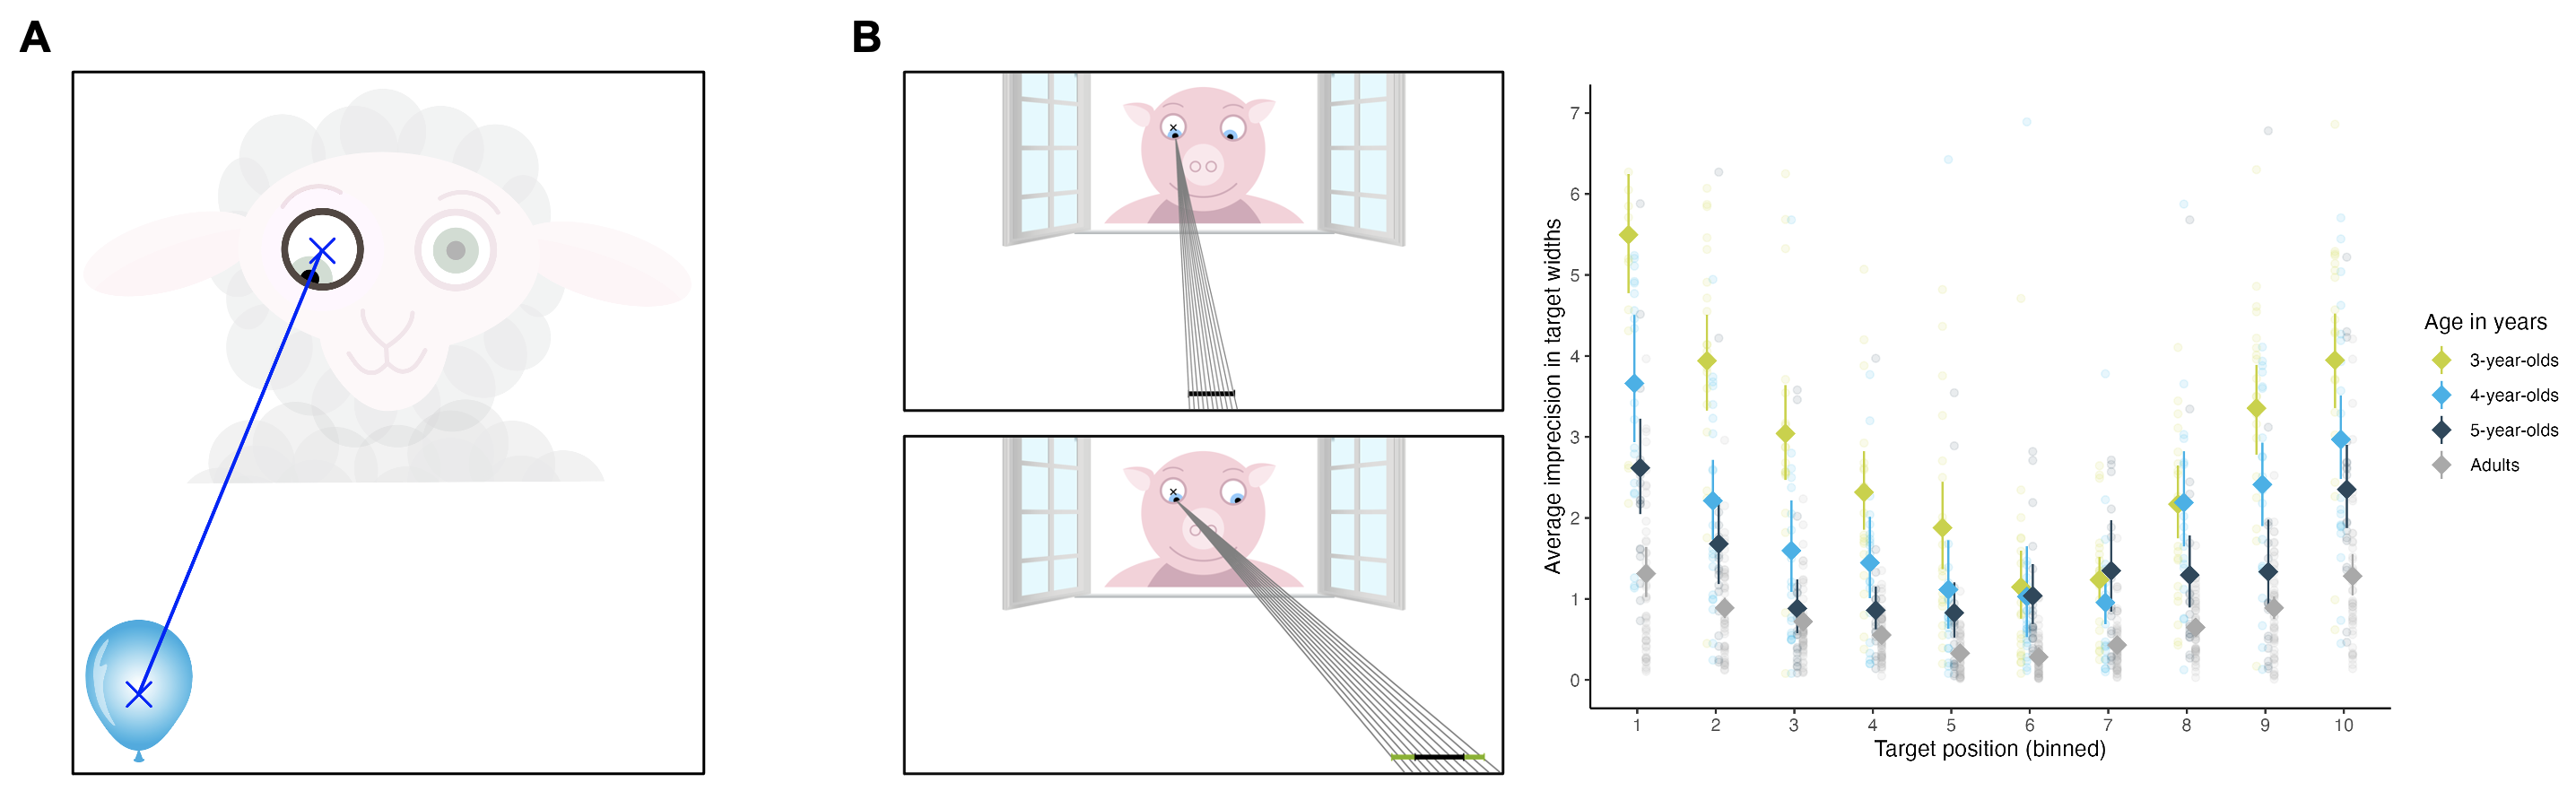
\includegraphics[width=1\linewidth]{../figures/gazefunnel_combined} 

}

\caption{\textbf{Gaze funnel}}\label{fig:fig3}
\end{figure}

\hypertarget{discussion-1}{%
\subsection{Discussion}\label{discussion-1}}

\hypertarget{components-of-gaze-understanding}{%
\section{Components of gaze understanding}\label{components-of-gaze-understanding}}

Our computational cognitive model assumes that the ability to engage in vector estimation is a crucial component of mastering gaze understanding.
In this study, we sought to experimentally isolate the physical vector estimation component.
In addition, we inquired whether there are any other cognitive processes outside the vector estimation that constitute gaze understanding.
We aimed to assess whether there are exclusively task-specific processes at hand or whether gaze understanding recruits a general social-cognitive ability that is shared among other social-cognitive tasks.

First, we aimed to isolate the vector estimation component of the gaze understanding task.
We designed a new non-social vector estimation task that shared all crucial design features of the gaze understanding task.
Second, we assessed children's social-cognitive abilities by administering a ToM task battery, comprising four tasks from the ToM scale by Wellman and Liu (Wellman and Liu (2004)) and two additional perspective-taking tasks (Flavell, Everett, Croft, \& Flavell, 1981; Flavell, Flavell, Green, \& Wilcox, 1981).

Our reasoning was that the gaze understanding task shares task demands with the non-social vector estimation task, while it shares its social context with the ToM tasks.
This way, we can disentangle what components comprise gaze understanding.

Task design, data collection, and sample sizes were pre-registered: \url{https://osf.io/xsqkt}.
The study design and procedure obtained ethical clearance by the MPG Ethics commission Munich, Germany, falling under a packaged ethics application (Appl. No.~2021\_45), and was approved by an internal ethics committee at the Max Planck Institute for Evolutionary Anthropology.
The research adheres to the legal requirements of psychological research with children in Germany.
Data were collected between February and March 2023.

\hypertarget{participants-2}{%
\subsection{Participants}\label{participants-2}}

Testing took place in kindergartens in Leipzig, Germany.
The sample consisted of 102 children (mean age = 4.54 years, SD = 0.31, range = 3.99 - 5.03, 54 girls).
Information on individual socio-economic status was not formally recorded.
Children in our sample live in an industrialized, urban Central-European city with approximately 600,000 inhabitants.
Households often consist of nuclear families with few household members.
The majority of families in our data base come from mainly mid to high socio-economic backgrounds with high levels of parental education.

\hypertarget{procedure-2}{%
\subsection{Procedure}\label{procedure-2}}

Children were tested in a quiet room in their kindergarten.
An experimenter guided the child through the study.
Since our research questions related to individual differences and we wanted maximum control of extraneous participant variables, we employed a within-subjects study design.
All participants performed the following tasks in a fixed order: (1) non-social vector estimation task, (2) ToM task battery, (3) gaze understanding task.
Several reasons motivated this decision.
First, we decided on a fixed order to be able to compare participants' performance straight-forwardly with each other.
Second, to increase participant engagement and decrease fatigue or fuzziness, we switched from a tablet task to tasks with personal interaction back to a tablet task.
Third, we showed the non-social vector estimation task before the gaze understanding task so that participants would not be biased to interpret the presented stimuli as ``eye- /''agent-like''.

\hypertarget{non-social-vector-estimation}{%
\subsubsection{Non-social vector estimation}\label{non-social-vector-estimation}}

Modeling the setup and structure of the previously applied gaze understanding task, we designed a non-social vector estimation task.
This task was also presented as a webapp on a tablet and made use of the concept of magnetism.
The setup looked as follows.
On the upper part of the screen, there was a tube with a gearwheel located in a circular window.
On the floor, there lay a magnet.
The magnet then got switched on (making a cartoon-like sound), whereupon the gearwheel moved towards the magnet.
The gearwheel moved in a way that its center aligned with the center of the magnet, while staying inside the circular window.
Participants were then asked to locate the magnet.
Access to the magnet's true location was manipulated by a wooden wall: participants either had full, partial, or no visual access to the true magnet location.
When no information about the magnet location was accessible, participants were expected to use the gearwheel inside the window as a non-social cue to locate the magnet.

As in the TANGO, there were three different trial types depending on the visual access to the true magnet location.
In full visual access trials, the magnet's location was presented without impediment (i.e., no wooden wall).
In partial visual access trials, the wooden wall was moved in front of the target after the magnet's location had already been visible.
In test trials, participants had no visual access to the magnet's location because the wall covered the magnet from the beginning of the trial.

Children received 19 trials with one full visual access trial, two partial visual access trials, and 16 test trials.
The first trial of each type comprised a voice-over description of the presented events.
We conducted our analysis with 15 test trials (excluding the voice-over trial).
The outcome variable was imprecision, defined as the absolute difference between the magnet's x coordinate and the x coordinate of the participant's click.
Magnet coordinates were generated as follows.
The full width of the screen was divided into ten bins.
Each bin occurred equally often, while the same bin could occur in two consecutive trials.
Exact coordinates within each bin were randomly generated.

\hypertarget{theory-of-mind-task-battery}{%
\subsubsection{Theory of Mind task battery}\label{theory-of-mind-task-battery}}

We administered four tasks from the Wellman and Liu (2004) Theory of Mind scale.
We excluded three tasks: the Diverse Desires task in order to avoid ceiling effects; and both tasks involving emotions (Belief Emotion and Real-Apparent Emotion), as we aimed at assessing the ``cold, cognitive'' (as compared to the ``emotional'') aspects of social cognition.
Instead, we added two perspective-taking level-2 tasks (Flavell, Everett, et al., 1981; Flavell, Flavell, et al., 1981).
We added the perspective-taking tasks (1) with the aim of increasing the task battery's difficulty, and (2) since we hypothesized that perspective-taking would rely on similar mechanisms than gaze understanding.
The dependent variable was the aggregate score of all solved ToM tasks (see Supplements for further detail).
In an exploratory analysis, we investigated if gaze understanding was more strongly associated with the two perspective-taking tasks compared to the other ToM tasks, as perspective-taking seems most closely theoretically related to gaze understanding (i.e., in both cases the participant is asked to judge another person's point of view).

\hypertarget{gaze-understanding}{%
\subsubsection{Gaze understanding}\label{gaze-understanding}}

As in the two previously reported studies, we presented children with the continuous version of the TANGO (Prein et al., 2022).
To accentuate the social aspect of the gaze understanding task, we exchanged the animal agents (used in the previous two studies) with human faces, which were modeled after the local population in appearance (already created for another project on cross-cultural similarities in gaze understanding (\url{https://osf.io/tdsvc})).
This further highlighted the contrast (i.e., social vs.~non-social context) to the non-social vector estimation task.\footnote{In an exploratory analysis, we compared children's imprecision levels in the TANGO task with animal vs.~human agents.
  Based on a GLMM analysis, we conclude that there was no evidence of a stable effect of stimulus choice (human vs.~animal).
  See Supplements for further detail.}

\hypertarget{analysis-2}{%
\subsection{Analysis}\label{analysis-2}}

By design, both the gaze understanding task as well as the non-social vector estimation task involve vector estimation.
On the basis of the results from our computational cognitive model, we expected that children's performance in both tasks correlate with each other.
For each of these two tasks, we calculated the mean level of imprecision for each subject.
We then correlated these two scores using \emph{Pearson's} correlation coefficients.

Regarding the relationship between the two vector estimation tasks and the ToM measures, we could imagine two possible scenarios: (A) If gaze understanding recruits a general social-cognitive ability beyond vector estimation, we expected that gaze understanding and ToM measures would correlate more strongly with each other than non-social vector estimation and ToM measures.
(B) If gaze understanding relies purely on task-specific processes, then the correlation between gaze understanding and ToM measures would be comparable to the correlation between non-social vector estimation and the ToM measures.
For the association between the aggregate ToM scores and the gaze understanding / non-social vector estimation tasks, we used \emph{Spearman's} rank correlation coefficients.

We compared the correlation between gaze understanding and ToM measures and the correlation between non-social vector estimation and ToM measures by using the Williams' test from the function \texttt{cocor.dep.groups.overlap} (designed for two dependent overlapping correlations) from the package \texttt{cocor} (Diedenhofen \& Musch, 2015).

Furthermore, to estimate which components best explain the gaze understanding score, we conducted a model comparison with GLMMs predicting the mean imprecision in gaze understanding by age, imprecision in non-social vector estimation, the ToM aggregate score, or the aggregate of the two perspective-taking tasks (subset of ToM battery; example of model notation in \texttt{R:\ tango\_mean\ \textasciitilde{}\ age\_centered\ +\ magnet\_scaled\ +\ perspective\_scaled}).
We wanted to assess whether the ToM aggregate score or the singled-out perspective-taking score added additional explanatory value when predicting the gaze understanding score.
The outcome variable was modeled by a lognormal distribution.

\hypertarget{results-2}{%
\subsection{Results}\label{results-2}}

As expected, we found that gaze understanding as a social vector estimation task correlated with the non-social vector estimation task, \emph{r} = 0.38, 95\%CI {[}0.20, 0.53{]}.
Importantly, however, the two vector estimation tasks were not redundant: only a part of the variance in gaze understanding could be explained by non-social vector estimation.

Gaze understanding and perspective-taking showed a \emph{Spearman} correlation coefficient of \(\rho\) = -0.29, 95\%CI {[}-0.46, -0.10{]}, while non-social vector estimation and perspective-taking did not correlate, \(\rho\) = -0.09, 95\%CI {[}-0.28, 0.10{]}.
According to the Williams' test, these two correlations did not differ significantly from each other, \emph{t}(99) = -1.86, \emph{p} = 0.07.

Our model comparison revealed that gaze understanding was best predicted by a model including non-social vector estimation (\(\beta\) = 0.14, 95\% CrI {[}0.06; 0.21{]}) and perspective-taking (\(\beta\) = -0.10; 95\% CrI {[}-0.17, -0.03{]}), even when controlling for age (\(\beta\) = -0.14, 95\% CrI {[}-0.38, 0.10{]}).
See Supplements for further detail of the model comparison.

Taken together, this shows that the gaze understanding task recruited social-cognitive abilities beyond vector estimation.
Evidently, it shared some of its variance with other level 2 perspective-taking tasks, while the overall ToM aggregate score did not add explanatory power.



\begin{figure}

{\centering 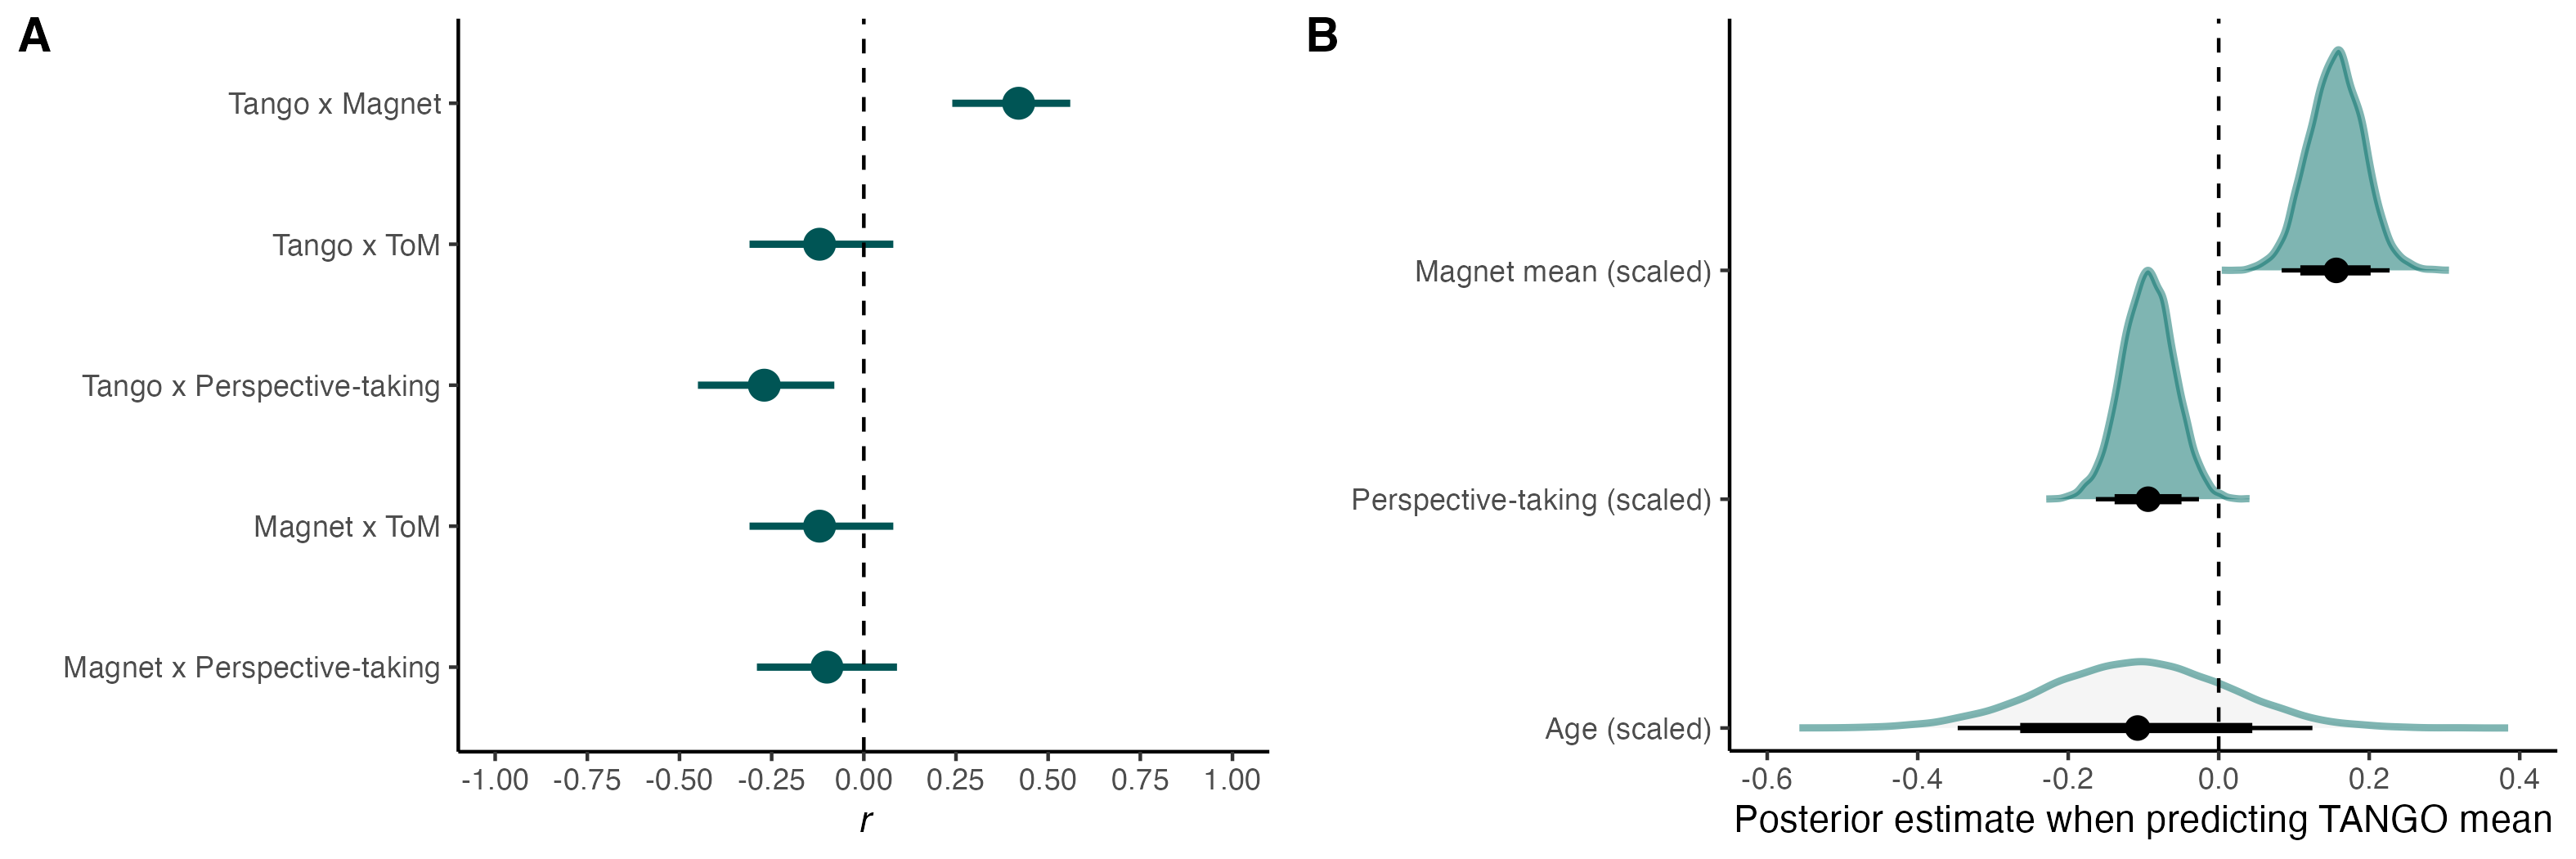
\includegraphics[width=1\linewidth]{../figures/magnet_arrangedplot} 

}

\caption{\textbf{Components of gaze understanding.} (A) Correlations between gaze understanding, physical vector estimation, ToM, and perspective-taking. Dots show the correlation coefficients, while error bars represent 95\% CIs. (B) Influence of perspective-taking and physical vector estimation on gaze understanding. The graph show the posterior distributions for the respective predictor. Black dots represent means, thicker black lines 80\% CrI and thinner black lines 95\% CrI.}\label{fig:fig4}
\end{figure}

\hypertarget{discussion-2}{%
\subsection{Discussion}\label{discussion-2}}

By carefully isolating physical vector estimation experimentally, we could show that gaze understanding does indeed, to a certain degree, rely on this component.
This is in line with our computational cognitive framework that assumes vector calculations on a process-level.
However, physical vector estimation alone did not suffice to explain gaze understanding.
In addition, perspective-taking proved to be a relevant social-cognitive ability.

In previous work, we could establish that the TANGO is suited as an individual differences measure (Prein et al., 2022).
Capturing meaningful variability in performance is a crucial task feature when we are interested in revealing the relationship between different cognitive abilities.
Importantly, the tasks we used to measure ToM abilities were not designed to capture individual differences: they relied on an aggregate score of dichotomous measures.
These sum scores can only capture limited variance, which may obscure potential correlations.
However, since these tasks are the gold standard in the social-cognitive literature and continuous measures with satisfying psychometric properties are, to the best of our knowledge, still scarce, we nonetheless relied on them in this study.
It seems noteworthy to point out that lower correlations between ToM abilities and gaze understanding could be grounded in the design features of the applied ToM tasks.
We already stated this concern in the Pre-registration (\url{https://osf.io/xsqkt}).
The development of new measures to capture individual differences in social-cognitive abilities like false-belief understanding seems desirable and essential to move this line of research further.

\hypertarget{general-discussion}{%
\section{General discussion}\label{general-discussion}}

\hypertarget{limitations}{%
\section{Limitations}\label{limitations}}

\hypertarget{conclusion}{%
\section{Conclusion}\label{conclusion}}

\newpage

\hypertarget{declarations}{%
\section{Declarations}\label{declarations}}

\hypertarget{open-practices-statement}{%
\subsection{Open practices statement}\label{open-practices-statement}}

The web application (\url{https://ccp-odc.eva.mpg.de/tango-demo/}) described here is open source (\url{https://github.com/ccp-eva/tango-demo}).
The data sets generated during and/or analysed during the current study are available in the {[}gazecues-modeling{]} repository (\url{https://github.com/ccp-eva/gazecues-modeling}).
All experiments were pre-registered (\url{https://osf.io/zjhsc/}).

\hypertarget{funding}{%
\subsection{Funding}\label{funding}}

This study was funded by the Max Planck Society for the Advancement of Science, a noncommercial, publicly financed scientific organization (no grant number).
We thank all the children, caregivers, and adults who participated in the study.
We thank Jana Jurkat for her help with data collection.

\hypertarget{conflicts-of-interest}{%
\subsection{Conflicts of interest}\label{conflicts-of-interest}}

The authors declare that they have no conflict of interest.

\hypertarget{consent-to-participate}{%
\subsection{Consent to participate}\label{consent-to-participate}}

Informed consent was obtained from all individual participants included in the study or their legal guardians.

\hypertarget{authors-contributions}{%
\subsection{Authors' contributions}\label{authors-contributions}}

The authors made the following contributions: \#\#\# TODO

\newpage

\hypertarget{references}{%
\section{References}\label{references}}

\begingroup
\setlength{\parindent}{-0.5in}
\setlength{\leftskip}{0.5in}

\hypertarget{refs}{}
\begin{CSLReferences}{1}{0}
\leavevmode\vadjust pre{\hypertarget{ref-astor2022gaze}{}}%
Astor, K., \& Gredebäck, G. (2022). Gaze following in infancy: {Five} big questions that the field should answer. In \emph{Advances in {Child Development} and {Behavior}} (p. S0065240722000192). {Elsevier}. \url{https://doi.org/10.1016/bs.acdb.2022.04.003}

\leavevmode\vadjust pre{\hypertarget{ref-behne2005oneyearolds}{}}%
Behne, T., Carpenter, M., \& Tomasello, M. (2005). One-year-olds comprehend the communicative intentions behind gestures in a hiding game. \emph{Developmental Science}, \emph{8}(6), 492--499. \url{https://doi.org/10.1111/j.1467-7687.2005.00440.x}

\leavevmode\vadjust pre{\hypertarget{ref-brooks2002importance}{}}%
Brooks, R., \& Meltzoff, A. N. (2002). The importance of eyes: {How} infants interpret adult looking behavior. \emph{Developmental Psychology}, \emph{38}(6), 958--966. \url{https://doi.org/10.1037/0012-1649.38.6.958}

\leavevmode\vadjust pre{\hypertarget{ref-burkner2017brms}{}}%
Bürkner, P.-C. (2017). Brms: {An R Package} for {Bayesian Multilevel Models Using Stan}. \emph{Journal of Statistical Software}, \emph{80}(1), 1--28. \url{https://doi.org/10.18637/jss.v080.i01}

\leavevmode\vadjust pre{\hypertarget{ref-burkner2018advanced}{}}%
Bürkner, P.-C. (2018). Advanced {Bayesian Multilevel Modeling} with the {R Package} brms. \emph{The R Journal}, \emph{10}(1), 395. \url{https://doi.org/10.32614/RJ-2018-017}

\leavevmode\vadjust pre{\hypertarget{ref-butterworth1991minds}{}}%
Butterworth, G., \& Jarrett, N. (1991). What minds have in common is space: {Spatial} mechanisms serving joint visual attention in infancy. \emph{British Journal of Developmental Psychology}, \emph{9}(1), 55--72. \url{https://doi.org/10.1111/j.2044-835X.1991.tb00862.x}

\leavevmode\vadjust pre{\hypertarget{ref-carpenter1998social}{}}%
Carpenter, M., Nagell, K., \& Tomasello, M. (1998). \href{https://www.ncbi.nlm.nih.gov/pubmed/9835078}{Social cognition, joint attention, and communicative competence from 9 to 15 months of age}. \emph{Monographs of the Society for Research in Child Development}, \emph{63}(4), i--vi, 1--143.

\leavevmode\vadjust pre{\hypertarget{ref-coelho2006searching}{}}%
Coelho, E., George, N., Conty, L., Hugueville, L., \& Tijus, C. (2006). Searching for asymmetries in the detection of gaze contact versus averted gaze under different head views: A behavioural study. \emph{Spatial Vision}, \emph{19}(6), 529--545. \url{https://doi.org/10.1163/156856806779194026}

\leavevmode\vadjust pre{\hypertarget{ref-colombo2001development}{}}%
Colombo, J. (2001). The development of visual attention in infancy. \emph{Annual Review of Psychology}, \emph{52}, 337--367. \url{https://doi.org/10.1146/annurev.psych.52.1.337}

\leavevmode\vadjust pre{\hypertarget{ref-dentremont1997demonstration}{}}%
D'Entremont, B., Hains, S. M. J., \& Muir, D. W. (1997). A demonstration of gaze following in 3- to 6-month-olds. \emph{Infant Behavior and Development}, \emph{20}(4), 569--572. \url{https://doi.org/10.1016/S0163-6383(97)90048-5}

\leavevmode\vadjust pre{\hypertarget{ref-diedenhofen2015cocor}{}}%
Diedenhofen, B., \& Musch, J. (2015). Cocor: {A Comprehensive Solution} for the {Statistical Comparison} of {Correlations}. \emph{PLoS ONE}, \emph{10}(4), e0121945. \url{https://doi.org/10.1371/journal.pone.0121945}

\leavevmode\vadjust pre{\hypertarget{ref-flavell1981younga}{}}%
Flavell, J. H., Everett, B. A., Croft, K., \& Flavell, E. R. (1981). Young children's knowledge about visual perception: {Further} evidence for the {Level} 1\textendash{{Level}} 2 distinction. \emph{Developmental Psychology}, \emph{17}, 99--103. \url{https://doi.org/10.1037/0012-1649.17.1.99}

\leavevmode\vadjust pre{\hypertarget{ref-flavell1981development}{}}%
Flavell, J. H., Flavell, E. R., Green, F. L., \& Wilcox, S. A. (1981). The {Development} of {Three Spatial Perspective-Taking Rules}. \emph{Child Development}, \emph{52}(1), 356--358. \url{https://doi.org/10.2307/1129250}

\leavevmode\vadjust pre{\hypertarget{ref-frischen2007gaze}{}}%
Frischen, A., Bayliss, A. P., \& Tipper, S. P. (2007). Gaze cueing of attention: {Visual} attention, social cognition, and individual differences. \emph{Psychological Bulletin}, \emph{133}(4), 694--724. \url{https://doi.org/10.1037/0033-2909.133.4.694}

\leavevmode\vadjust pre{\hypertarget{ref-gathercole2004structure}{}}%
Gathercole, S. E., Pickering, S. J., Ambridge, B., \& Wearing, H. (2004). The {Structure} of {Working Memory From} 4 to 15 {Years} of {Age}. \emph{Developmental Psychology}, \emph{40}, 177--190. \url{https://doi.org/10.1037/0012-1649.40.2.177}

\leavevmode\vadjust pre{\hypertarget{ref-grahek2021anatomy}{}}%
Grahek, I., Schaller, M., \& Tackett, J. L. (2021). Anatomy of a {Psychological Theory}: {Integrating Construct-Validation} and {Computational-Modeling Methods} to {Advance Theorizing}. \emph{Perspectives on Psychological Science}, \emph{16}(4), 803--815. \url{https://doi.org/10.1177/1745691620966794}

\leavevmode\vadjust pre{\hypertarget{ref-itakura1998use}{}}%
Itakura, S., \& Tanaka, M. (1998). Use of experimenter-given cues during object-choice tasks by chimpanzees ({Pan} troglodytes), an orangutan ({Pongo} pygmaeus), and human infants ({Homo} sapiens). \emph{Journal of Comparative Psychology}, \emph{112}(2), 119--126. \url{https://doi.org/10.1037/0735-7036.112.2.119}

\leavevmode\vadjust pre{\hypertarget{ref-lee1998children}{}}%
Lee, K., Eskritt, M., Symons, L. A., \& Muir, D. (1998). Children's use of triadic eye gaze information for "mind reading". \emph{Developmental Psychology}, \emph{34}(3), 525--539. \url{https://doi.org/10.1037//0012-1649.34.3.525}

\leavevmode\vadjust pre{\hypertarget{ref-moll200412}{}}%
Moll, H., \& Tomasello, M. (2004). 12- and 18-month-old infants follow gaze to spaces behind barriers. \emph{Developmental Science}, \emph{7}(1), F1--F9. \url{https://doi.org/10.1111/j.1467-7687.2004.00315.x}

\leavevmode\vadjust pre{\hypertarget{ref-moore1997role}{}}%
Moore, C., Angelopoulos, M., \& Bennett, P. (1997). The role of movement in the development of joint visual attention. \emph{Infant Behavior and Development}, \emph{20}(1), 83--92. \url{https://doi.org/10.1016/S0163-6383(97)90063-1}

\leavevmode\vadjust pre{\hypertarget{ref-palan2018prolific}{}}%
Palan, S., \& Schitter, C. (2018). Prolific.ac\textemdash{{A}} subject pool for online experiments. \emph{Journal of Behavioral and Experimental Finance}, \emph{17}, 22--27. \url{https://doi.org/10.1016/j.jbef.2017.12.004}

\leavevmode\vadjust pre{\hypertarget{ref-povinelli1997exploitation}{}}%
Povinelli, D. J., Reaux, J. E., Bierschwale, D. T., Allain, A. D., \& Simon, B. B. (1997). Exploitation of pointing as a referential gesture in young children, but not adolescent chimpanzees. \emph{Cognitive Development}, \emph{12}(4), 423--461. \url{https://doi.org/10.1016/S0885-2014(97)90017-4}

\leavevmode\vadjust pre{\hypertarget{ref-prein2022tango}{}}%
Prein, J. C., Bohn, M., Kalinke, S., \& Haun, D. B. M. (2022). \emph{{TANGO}: {A} reliable, open-source, browser-based task to assess individual differences in gaze understanding in 3 to 5-year-old children and adults}. {PsyArXiv}. \url{https://doi.org/10.31234/osf.io/vghw8}

\leavevmode\vadjust pre{\hypertarget{ref-rcoreteam2022language}{}}%
R Core Team. (2022). \emph{R: {A} language and environment for statistical computing} {[}Manual{]}. {Vienna, Austria}: {R Foundation for Statistical Computing}.

\leavevmode\vadjust pre{\hypertarget{ref-raviv2018developmental}{}}%
Raviv, L., \& Arnon, I. (2018). The developmental trajectory of children's auditory and visual statistical learning abilities: Modality-based differences in the effect of age. \emph{Developmental Science}, \emph{21}(4), e12593. \url{https://doi.org/10.1111/desc.12593}

\leavevmode\vadjust pre{\hypertarget{ref-scaife1975capacity}{}}%
Scaife, M., \& Bruner, J. S. (1975). The capacity for joint visual attention in the infant. \emph{Nature}, \emph{253}(5489), 265--266. \url{https://doi.org/10.1038/253265a0}

\leavevmode\vadjust pre{\hypertarget{ref-silverstein2021infants}{}}%
Silverstein, P., Feng, J., Westermann, G., Parise, E., \& Twomey, K. E. (2021). Infants {Learn} to {Follow Gaze} in {Stages}: {Evidence Confirming} a {Robotic Prediction}. \emph{Open Mind}, \emph{5}, 174--188. \url{https://doi.org/10.1162/opmi_a_00049}

\leavevmode\vadjust pre{\hypertarget{ref-simmering2010dialogue}{}}%
Simmering, V. R., Triesch, J., Deák, G. O., \& Spencer, J. P. (2010). A {Dialogue} on the {Role} of {Computational Modeling} in {Developmental Science}. \emph{Child Development Perspectives}, \emph{4}(2), 152--158. \url{https://doi.org/10.1111/j.1750-8606.2010.00134.x}

\leavevmode\vadjust pre{\hypertarget{ref-tomasello2007reliance}{}}%
Tomasello, M., Hare, B., Lehmann, H., \& Call, J. (2007). Reliance on head versus eyes in the gaze following of great apes and human infants: The cooperative eye hypothesis. \emph{Journal of Human Evolution}, \emph{52}(3), 314--320. \url{https://doi.org/10.1016/j.jhevol.2006.10.001}

\leavevmode\vadjust pre{\hypertarget{ref-wellman2004scaling}{}}%
Wellman, H. M., \& Liu, D. (2004). Scaling of {Theory-of-Mind Tasks}. \emph{Child Development}, \emph{75}(2), 523--541. \url{https://doi.org/10.1111/j.1467-8624.2004.00691.x}

\leavevmode\vadjust pre{\hypertarget{ref-zhang2019role}{}}%
Zhang, X., Zhang, Z., Zhang, Z., Tang, Y., \& Liu, W. (2019). The role of the motion cue in the dynamic gaze-cueing effect: {A} study of the lateralized {ERPs}. \emph{Neuropsychologia}, \emph{124}, 151--160. \url{https://doi.org/10.1016/j.neuropsychologia.2018.12.016}

\end{CSLReferences}

\endgroup

\newpage


\end{document}
